%\documentclass[12pt,modern,twocolumn,tighten]{aastex63}
%\documentclass[12pt,twocolumn]{aastex63}
%\documentclass[12pt,modern,twocolumn,tighten,linenumbers,trackchanges]{aastex63}
\documentclass[12pt,tighten,linenumbers]{aastex63}
%\documentclass[12pt,twocolumn,tighten,linenumbers,trackchanges]{aastex63}
\usepackage{amsmath,amstext,amssymb}
\usepackage[T1]{fontenc}
\usepackage{apjfonts}
\usepackage[figure,figure*]{hypcap}
\usepackage{graphics,graphicx}
\usepackage{hyperref}
\usepackage{natbib}
\usepackage[caption=false]{subfig} % for subfloat
\usepackage{enumitem} % for specific spacing of enumerate
\usepackage{epigraph}

\renewcommand*{\sectionautorefname}{Section} %for \autoref
\renewcommand*{\subsectionautorefname}{Section} %for \autoref

\newcommand{\cn}{Cep-Her complex} % cluster name
\newcommand{\sysone}{Kepler-1627} % star system name (binary)
\newcommand{\stone}{Kepler-1627 A} % star system name (binary)
\newcommand{\plone}{Kepler-1627 Ab} % planet name
\newcommand{\systwo}{Kepler-1643} % star system name (binary)
\newcommand{\sttwo}{Kepler-1643} % star system name (binary)
\newcommand{\pltwo}{Kepler-1643 b} % planet name
\newcommand{\systhree}{KOI-7368} % star system name (binary)
\newcommand{\stthree}{KOI-7368} % star system name (binary)
\newcommand{\plthree}{KOI-7368 b} % planet name
\newcommand{\sysfour}{KOI-7913 } % star system name (binary)
\newcommand{\stfour}{KOI-7913 A} % star system name (binary)
\newcommand{\plfour}{KOI-7913 Ab} % planet name

\newcommand{\clusterage}{$38^{+6}_{-5}$\,Myr} % 

\newcommand{\npms}{1{,}097} % 20220311_Kerr_SPYGLASS205_Members_All.csv
\newcommand{\nchtwo}{37} % CH-2_auto_XYZ_vl_vb_cut.csv
\newcommand{\nrsgfive}{173} % RSG-5_auto_XYZ_vl_vb_cut.csv

%
% Symbols
%
\newcommand{\kms}{\,km\,s$^{-1}$}
\newcommand{\mkms}{{\rm \,km\,s^{-1}}}  % math mode
\newcommand{\ms}{\,m\,s$^{-1}$}
\newcommand{\bpmrpo}{(G_{\rm BP}-G_{\rm RP})_0}
\newcommand{\bpmrp}{G_{\rm BP}-G_{\rm RP}}

%% Reintroduced the \received and \accepted commands from AASTeX v5.2.
%% Add "Submitted to " argument.
%\received{2022 May 2}
%\revised{2022 Sep 14}
%\accepted{2022 Sep 17}
\submitjournal{Astronomical Journal}
\shorttitle{Kepler and the Behemoth}

\begin{document}

\title{
  Erratum: ``Kepler and the Behemoth: Three Mini-Neptunes in a 40 Million Year Old Association'' (2022, AJ, 164, 215)
}

%\suppressAffiliations
%\NewPageAfterKeywords
\correspondingauthor{L.\,G.\,Bouma}
\email{bouma.luke@gmail.com}

\author[0000-0002-0514-5538]{L. G. Bouma}
\affiliation{Department of Astrophysical Sciences, Princeton University, 4 Ivy Lane, Princeton, NJ 08540, USA}

% Key authors:
% ... stellar rotation & the initial crossmatch
\author[0000-0002-2792-134X]{J. L. Curtis}
\affiliation{Department of Astronomy, Columbia University, 550 West 120th Street, New York, NY 10027, USA}
\affiliation{Department of Astrophysics, American Museum of Natural History, New York, NY 10024, USA}

% ... Kepler correlations
\author[0000-0003-1298-9699]{K. Masuda}
\affiliation{Department of Earth and Space Science, Osaka University, Osaka 560-0043, Japan}

% ... HIRES PI
\author{L. A. Hillenbrand}
\affiliation{Cahill Center for Astrophysics, California Institute of Technology, Pasadena, CA 91125, USA}

% ... RM fitting
\author[0000-0001-7409-5688]{G. Stefansson}
\affiliation{Department of Astrophysical Sciences, Princeton University, 4 Ivy Lane, Princeton, NJ 08540, USA}

%
% PFS Collaborators
%
\author[0000-0001-8638-0320]{A. W. Howard}
\affiliation{Cahill Center for Astrophysics, California Institute of Technology, Pasadena, CA 91125, USA}
%
\author[0000-0002-0531-1073]{H. Isaacson}
\affiliation{Astronomy Department, University of California, Berkeley,
CA 94720, USA}

%
% MUSCAT3 Collaborators
%
\author[0000-0001-8511-2981]{N. Narita}
\affiliation{Komaba Institute for Science, The University of Tokyo, Tokyo 153-8902, Japan}
\affiliation{Japan Science and Technology Agency, PRESTO, Tokyo 153-8902, Japan}
\affiliation{Astrobiology Center, Tokyo 181-8588, Japan}
\affiliation{Instituto de Astrof\'{i}sica de Canarias (IAC), 38205 La Laguna, Tenerife, Spain}

\author[0000-0002-4909-5763]{A. Fukui} % afukui@g.ecc.u-tokyo.ac.jp
\affiliation{Komaba Institute for Science, The University of Tokyo, Tokyo 153-8902, Japan}
\affiliation{Instituto de Astrof\'{i}sica de Canarias (IAC), 38205 La Laguna, Tenerife, Spain}

\author[0000-0002-5658-5971]{Masahiro Ikoma} % ikoma.masahiro@gmail.com
\affiliation{Division of Science, National Astronomical Observatory of Japan, Tokyo 181-8588, Japan}

\author[0000-0002-6510-0681]{M. Tamura} % motohide.tamura@nao.ac.jp
\affiliation{Department of Astronomy, University of Tokyo, Tokyo 113-0033, Japan}
\affiliation{Astrobiology Center, Tokyo 181-8588, Japan}
\affiliation{National Astronomical Observatory of Japan, Tokyo 181-8588, Japan}

% AO IMAGING
\author[0000-0001-9800-6248]{E. Furlan} % furlan@ipac.caltech.edu
\affiliation{NASA Exoplanet Science Institute, Caltech/IPAC, Pasadena, CA 91125, USA}

\author[0000-0003-2519-6161]{C.~L.~Gnilka} % clgnilka@gmail.com
\affiliation{NASA Ames Research Center, Moffett Field, CA 94035, USA}

\author[0000-0002-9903-9911]{K.~V.~Lester} % klester192@gmail.com
\affiliation{NASA Ames Research Center, Moffett Field, CA 94035, USA}

\author[0000-0002-2532-2853]{S. B. Howell}
\affiliation{NASA Ames Research Center, Moffett Field, CA 94035, USA}





%%%%%%%%%%%%%%%%%%%%%%%%%%%%%%%%%%%%%%%%%%%%%%%%%%%%%%%%%%%%%%%%%%%%%%%%%%%%%%%

\section*{ }

In the original manuscript, the top-right panel of Figure~2
erroneously omitted KOI-7913~B due to an error in the plotting script.
Figure~\ref{fig:age} in this erratum corrects the omission.

\begin{figure*}[tp]
	\begin{center}
		\leavevmode
		\subfloat{
			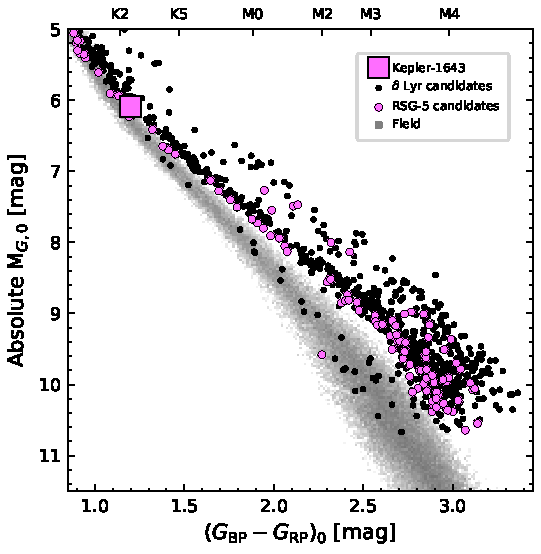
\includegraphics[width=0.49\textwidth]{f2a.pdf}
			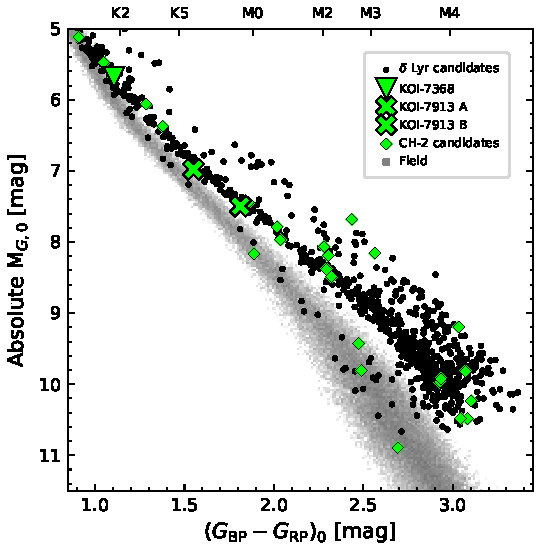
\includegraphics[width=0.49\textwidth]{f2b_corrected.pdf}
		}
		
		\vspace{-0cm}
		\subfloat{
			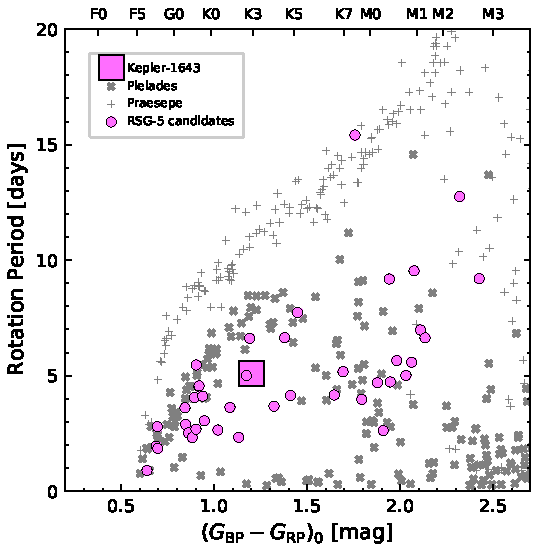
\includegraphics[width=0.49\textwidth]{f2c.pdf}
			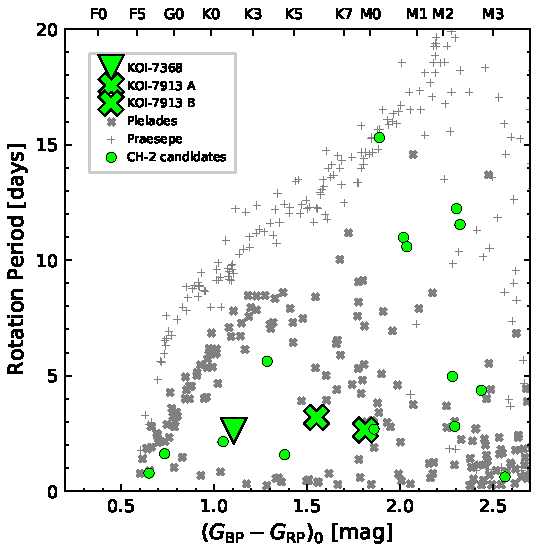
\includegraphics[width=0.49\textwidth]{f2d.pdf}
		}
	\end{center}
	\vspace{-0.5cm}
	\caption{
    {\bf Age-diagnostic diagrams from the stellar groups near
    Kepler-1643, KOI-7368, and KOI-7913.} 
    {\it Top row}: Color--absolute magnitude diagram of candidate
    Cep-Her members, plotted over candidate members of the
    $\delta$~Lyr~cluster ($\approx38$\,Myr;
    \citealt{bouma_kep1627_2022}) and the Gaia EDR3 Catalog of Nearby
    Stars (gray background).  The left and right columns shows stars
    in RSG-5 and CH-2, respectively.  The range of colors is truncated
    to emphasize the pre-main-sequence; approximate spectral types are
    shown on the upper axes.  Stars that fall far below the cluster
    sequences are field interlopers.  {\it Bottom row}: TESS and
    ZTF-derived stellar rotation periods, with the Pleiades ($\approx
    112$\,Myr) and Praesepe ($\approx 650$\,Myr) shown for reference
    \citep{rebull_rotation_2016a,douglas_poking_2017}.  The detection
    efficiency for reliable rotation periods falls off beyond $\bpmrpo
    \gtrsim 2.6$.
	\label{fig:age}
	}
\end{figure*}



\clearpage
\bibliographystyle{yahapj}                            
\bibliography{bibliography} 


%\clearpage
%\listofchanges
%\allauthors
\end{document}


